\subsection{What we call time}
A simple and intuitive way to introduce the NTK is via "\textbf{Gradient Flow}", which is an assumption related to the GD algorithm from \cref{sec:NetworkOptimization}. To quickly recap the update step from stochastic gradient descent, it is defined as 
\begin{equation}
	\theta' = \theta - \eta \nabla_\theta \mathscr{L}\left( \{(f_\theta(\mathbf{x}_i), \mathbf{y}_i)\}_{i=1}^{N} \right).
\end{equation}
The "flow" aspect arises when we start to ignore the discrete nature of these update steps and assume that the $\theta$ parameters change continuously by assuming $\eta \rightarrow 0$. A visual demonstration of how this changes the evolution of the parameters can be seen in \cref{fig:GradientFlowPlot}. The dashed markers represent the evolution under regular GD, while the solid line represents the evolution for gradient flow.
\begin{figure}
	\centering
	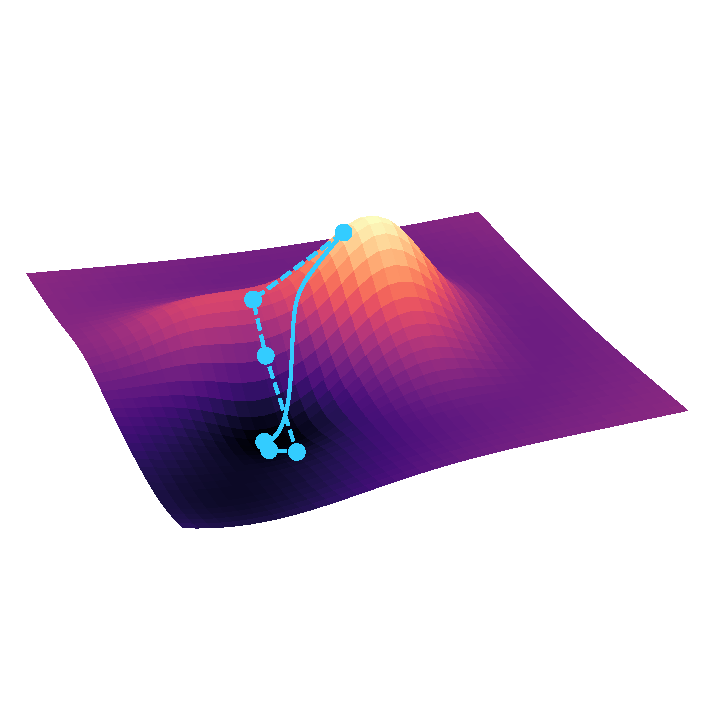
\includegraphics[width=12cm, clip, trim = 0cm 2.3cm 0cm 3.5cm]{text/NTK/GradientFlowPlot.pdf}
	\caption{This graph shows the difference between Gradient Descent and Gradient Flow. The dashed line along with the circle markers show the positions during regular GD with finite step sizes, the solid line shows the path of the parameters under gradient flow.}
	\label{fig:GradientFlowPlot}
\end{figure}
To do this, we first introduce a notion of "time" into our system. We try to visualize the optimization process as an evolution of our parameters $\theta$ through this variable called time, which converts updating the parameters into moving further along the timeline of our parameters. We translate $\theta \rightarrow \theta(t)$ and $\theta' \rightarrow \theta(t+\Delta t)$. This time in our system doesn't work exactly the same way as physical time, but since the process of optimizing parameters and changing them is always associated with the expenditure of physical time, it is intuitive to refer to our system's propagation variable as "time". \\
Returning to the GD algorithm, since the learning rate $\eta$ affects the size of our update step, we will refer to $\eta$ as the amount of time it takes to update a parameter $\theta' \rightarrow \theta(t+\eta)$. The whole GD algorithm then becomes
\begin{equation}
	\theta(t+\eta) = \theta(t) - \eta \nabla_{\theta(t)} \mathscr{L}\left( \{(f_{\theta(t)}(\mathbf{x}_i), \mathbf{y}_i)\}_{i=1}^{N} \right)
\end{equation}
which we can rewrite to 
\begin{equation}
	\frac{\theta(t+\eta)-\theta(t)}{\eta} = - \nabla_{\theta(t)} \mathscr{L}\left( \{(f_{\theta(t)}(\mathbf{x}_i), \mathbf{y}_i)\}_{i=1}^{N} \right).
\end{equation}
When observing the term on the left side, readers who are familiar with calculus might recognize that it looks similar to the definition of a derivative with respect to time when $\eta \rightarrow 0$
\begin{equation}
	\tAbl{}{t}\theta(t) = \lim_{\eta\rightarrow0} \frac{\theta(t+\eta)-\theta(t)}{\eta}.
\end{equation}
This means that for very infinitesimal learning rates we can approximate the GD as 
\begin{equation}\label{eq:NTKThetaDerivative}
	\tAbl{}{t}\theta(t) = - \nabla_{\theta(t)} \mathscr{L}\left( \{(f_{\theta(t)}(\mathbf{x}_i), \mathbf{y}_i)\}_{i=1}^{N} \right)
\end{equation}
with the derivative of $\theta$ along the assumed time variable.\\
For visual simplicity reasons, let's define the $j$-th component of the network output for the $i$-th input point $f_{\theta(t)}(\mathbf{x}_i)_j$ as $F_{ij}$ and assume Einstein summation for the rest of the chapter.
This means that when an index is occuring twice, we assume a hidden summation over all possible values for this index (for example $a_kb_k = \sum_k a_kb_k$).\\
Because it will be convenient later, we also spell out one component of the $\nabla_\theta$ derivation of the loss function further by using the chain rule as
\begin{align}
	\tAbl{\theta_k}{t} &= - \tAbl{}{\theta_k}\mathscr{L}\left( \{(f_{\theta(t)}(\mathbf{x}_i), \mathbf{y}_i)\}_{i=1}^{N} \right)\nonumber\\
	&= - \pAbl{\mathscr{L}}{F_{ij}} \cdot \tAbl{F_{ij}}{\theta_k}.
\end{align} 

\subsection{Derivation of the NTK}
This notion of time affects not only the parameters, but also everything that depends on them. For example, since the network output of a fixed architecture for a given input data point only depends on the parameters of the network, it can also be mathematically viewed as dependent on the time $f_{\theta}(\mathbf{x}_i) \rightarrow f_{\theta(t)}(\mathbf{x}_i)$. This means we can also calculate the derivative of one of the network outputs $f_{\theta(t)}(\mathbf{x}_i)_j = F_{ij}$ to
\begin{align}
	\tAbl{}{t} F_{ij} &= \pAbl{F_{ij}}{\theta_k}\tAbl{\theta_k}{t}\nonumber\\
	&= \pAbl{F_{ij}}{\theta_k} \left(- \pAbl{\mathscr{L}}{F_{ij}} \tAbl{F_{ij}}{\theta_k} \right)\label{eq:NTKarisesFromHere}\\
	&= - \underbrace{\pAbl{F_{ij}}{\theta_k} \pAbl{F_{lm}}{\theta_k}}_\mathlarger{=\vcentcolon \Lambda_{iljm}}
	\pAbl{\mathscr{L}}{F_{lm}}.\nonumber
\end{align}
In the last line, we used the fact that $F_{ij}$ explicitly depends on $\theta$, which means that the total and partial derivative ar interchangeable.
The rank 4 tensor $\Lambda$ is what we call the Neural Tangent Kernel for GD. We sorted the indices of this matrix so that the first two refer to the input points of $f$ and the last two refer to the components of the output dimensions of the neural network. Note that this NTK is derived directly from the update algorithm of the GD for infinitely small $\eta$ and only holds for linear gradient based algorithms.\\
Another way to derive the NTK using an approximation of $\Delta \mathscr{L}$ for small $\eta$ can be seen around page 196 of \cite{ThePrinciplesOfDeepLearningTheory}. The NTK is derived there in a more generic form using a learning rate tensor $\eta_{ij}$. Here it's important to note that the assumption of continuous parameter updates isn't necessary for the NTK. It also arises from the simple assumption of $\eta \rightarrow 0$, which makes it a viable observable for GD algorithms with small learning rates. 